%=================================================================
\section{Introduction}\label{sec-preliminaries}
\label{sec-intro}

In deep learning projects, data visualization operations often required include visualization of original image data, visualization of loss and accuracy, etc.Visualization abstracts Numbers into graphs that are more convenient for us to observe and feel. Through data visualization, data can be represented more intuitively.\\
  \indent In this study, the data in the data set are organized and analyzed to analyze the impact of commodity sales volume, product category, operating revenue and the economic scale of the city where the store is located on the revenue.The model was used to train the data set, the historical sales data was used as the characteristics of the model, and the sales results of this month were used as labels to build the model for regression analysis.\\
  \indent This paper This paper makes use of the existing methods to achieve the forecast of merchandise sales and effectively guide stores to carry out reasonable inventory management.It has good practical significance and application prospect.\\




















\section{Preliminaries} \label{sec-preliminaries}
The project aims to find out the relevant factors affecting the sales volume of goods, 
and predict the sales volume of different goods in the company's stores in the coming month.\\
Step 1:\\
Preprocessing of project data sets\\
Step 2:\\
Training set data cleaning\\
Through the data of the training set,we determined the parameters of the fitting curve. 
to filter the obvious outliers and checked the abnormal conditions of prices and sales\\ 
Step 3:\\
Structured data and analysis \\
This session includes sales analysis, profit analysis, view the overall sales trend.\\
analysis commodity sales products operating revenue and store city economic scale effect on revenue benefit.\\
Step 4:\\
Characteristics of the processing
Fuses the characteristics of the store data set and the merchandise data set.\\
Add sales characteristics and use the historical sales data as the characteristics of the model.\\
Step 5:\\
Model Adopted\\
This project uses lightGBM model for training.
%(1) Dataset Download:Download dataset from the kaggle project.\\
% \begin{center}
%   \begin{minipage}{0.3\linewidth}
%   \centering

%   \includegraphics[width=0.9\textwidth]{logos/21.eps}
 
%   {\small{Flag.1}}

%   \end{minipage}
%   \hfill
% \end{center}
% (2) Data cleaning: delete some unimportant or less influential data, such as poster_ path,overview,imdb_ ID, homepage, etc \\
% \begin{center}
%   \begin{minipage}{0.3\linewidth}
%   \centering

%   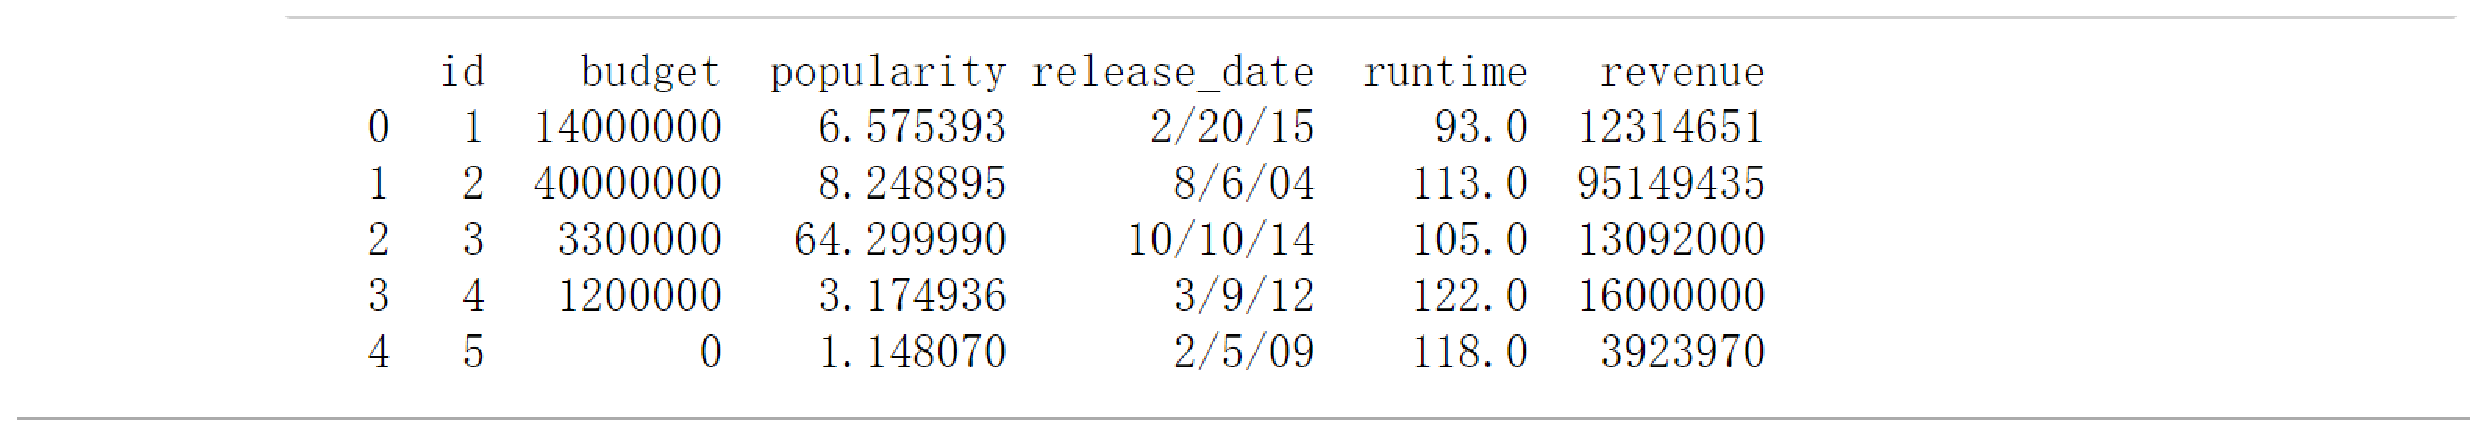
\includegraphics[width=0.9\textwidth]{logos/24.eps}
 
%   {\small{Flag.2}}

%   \end{minipage}
%   \hfill
% \end{center}
% (3) Data analysis: To observe the impact of previous investment on the film, we use Matplotlib in Python to draw a picture, flag 1, we can see that the investment is directly proportional to the business income.

% \begin{center}
%   \begin{minipage}{0.3\linewidth}
%   \centering

%   \includegraphics[width=0.9\textwidth]{logos/4.eps}
 
%   {\small{Flag.3}}

%   \end{minipage}
%   \hfill
% \end{center}

% To observe the impact of previous investment on the film, we use Matplotlib in Python to draw a picture, flag 1, we can see that the investment is directly proportional to the business income.

% \begin{center}
%   \begin{minipage}{0.3\linewidth}
%   \centering

%   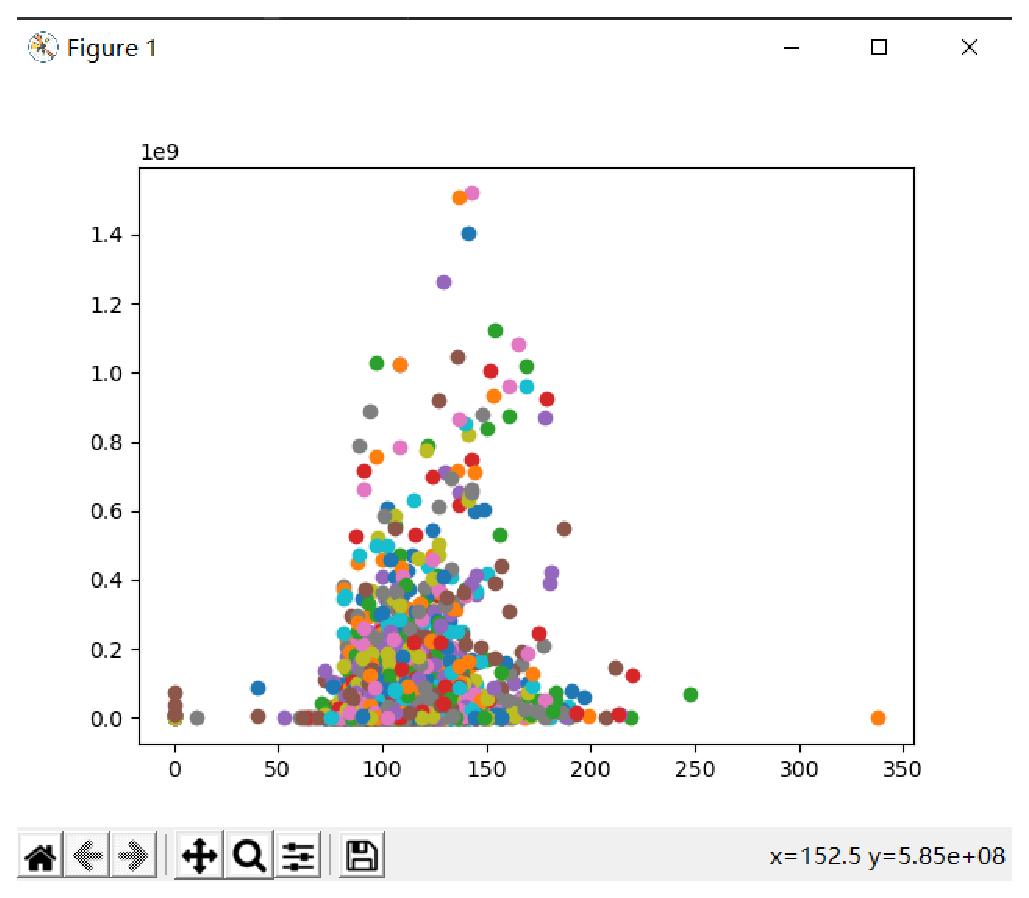
\includegraphics[width=0.9\textwidth]{logos/22.eps}
 
%   {\small{Flag.4}}

%   \end{minipage}
%   \hfill
% \end{center}
% To observe the impact of previous investment on the film, we use Matplotlib in Python to draw a picture, flag 1, we can see that the investment is directly proportional to the business income.

% \begin{center}
%   \begin{minipage}{0.3\linewidth}
%   \centering

%   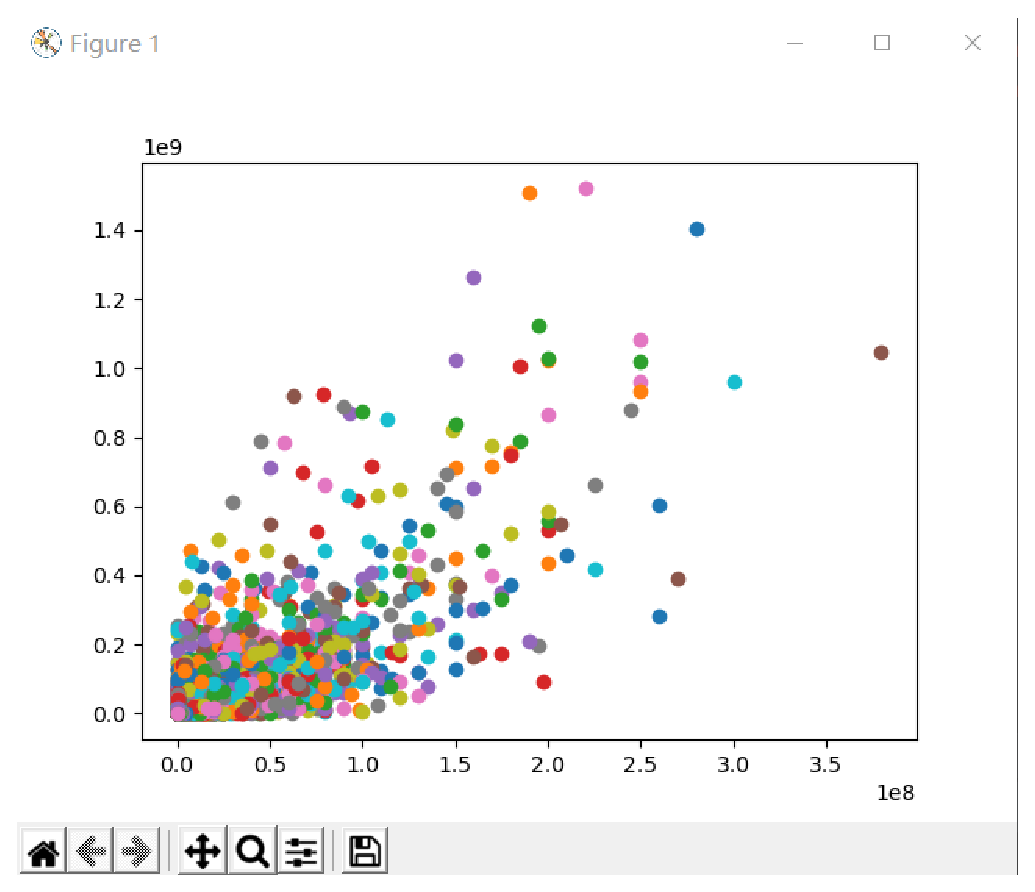
\includegraphics[width=0.9\textwidth]{logos/25.eps}
 
%   {\small{Flag.5}}

%   \end{minipage}
%   \hfill
% \end{center}
% To observe the impact of previous investment on the film, we use Matplotlib in Python to draw a picture, flag 1, we can see that the investment is directly proportional to the business income.

% \begin{center}

%   \begin{minipage}{0.3\linewidth}
%   \centering

%   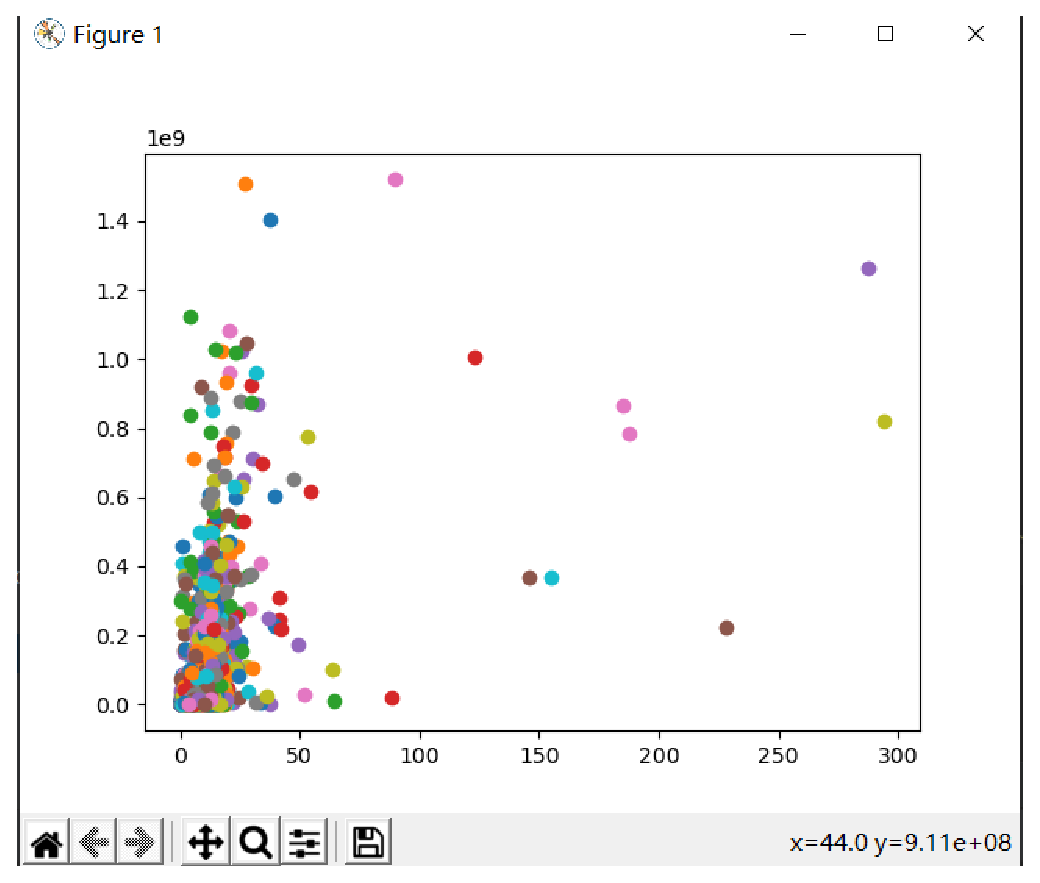
\includegraphics[width=0.9\textwidth]{logos/26.eps}
  
%   {\small{The relationship between popularity and business income}}

%   \end{minipage}
% \end{center}



\section{METHOD} \label{sec-experiment}
\indent In order to accurately predict the future sales of goods,this project uses LightGBM Model. \\
Before using the Model to train the data set, we need to conduct feature processing on the data set to get the expected results. \\
3.1 \textbf{Characteristics of the processing}\\
The goal is to use historical sales data to predict future sales.\\
Using the historical sales data as the characteristics of the model.\\
 this month's sales results as labels to build a model for regression analysis.\\
 3.2 \textbf{Model Adopted}\\
 This project uses lightGBM model for training.LightGBM is a fast, 
distributed, high-performance gradient enhancement framework based on 
decision tree algorithms.It supports category characteristics. \\
\indent LightGBM supports category characteristics directly and natively
by changing the decision rules of the decision tree algorithm, without transformation.
\begin{center}
  \begin{minipage}{0.5\linewidth}
  \centering
  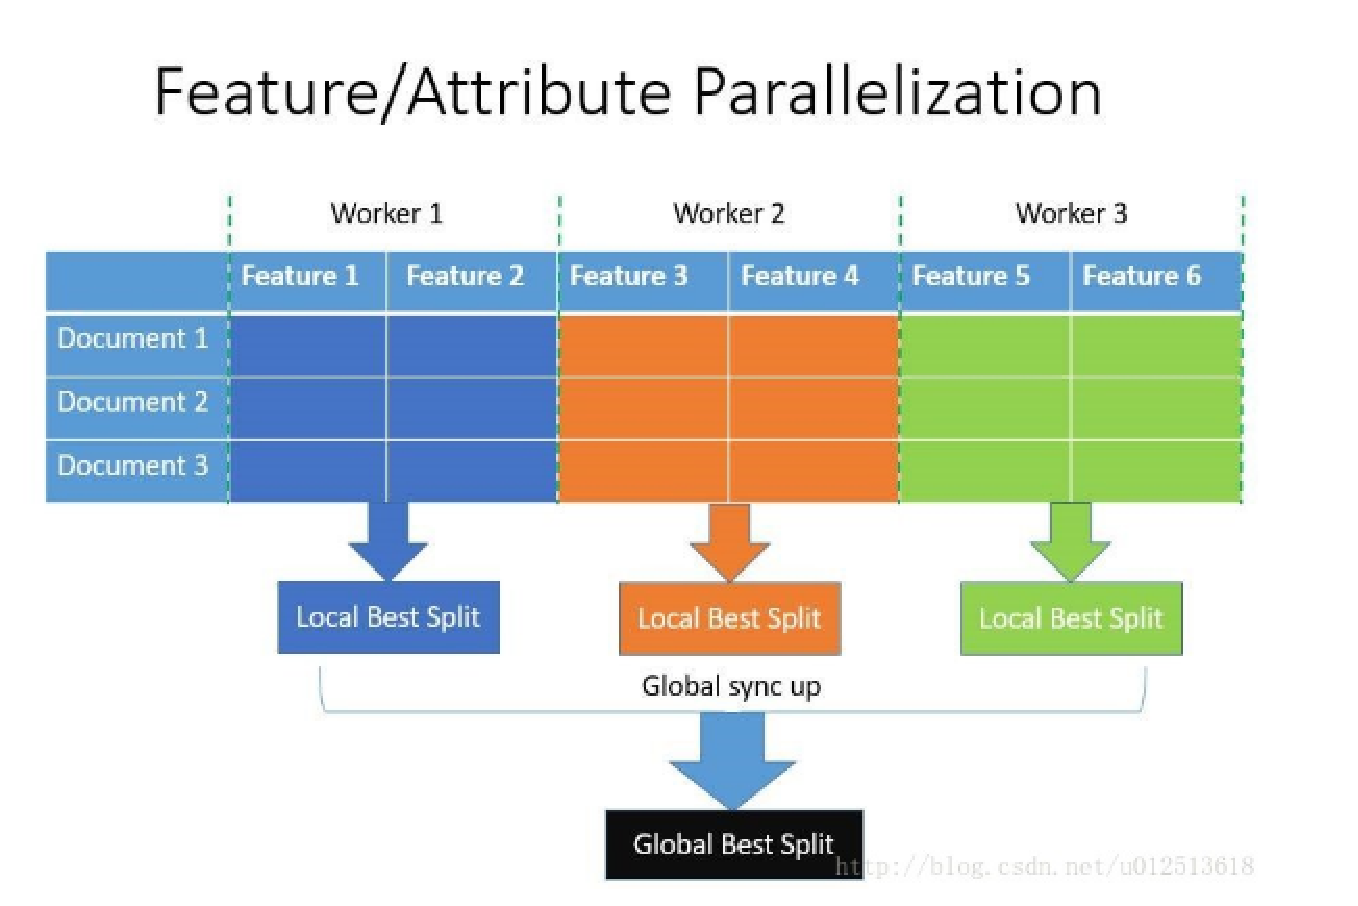
\includegraphics[width=1.1\textwidth]{logos/moxing.eps}
  \centering
  %{\small{cost}}
  \end{minipage}
\end{center}
% \begin{center}

%   \begin{minipage}{0.3\linewidth}
%   \centering

%   \includegraphics[width=0.9\textwidth]{logos/7.eps}
  
%   {\small{The relationship between popularity and business income}}

%   \end{minipage}
% \end{center}


% 3.1 parameter learning \\
% From the data analysis, we select several parameters which have the greatest impact on the business income as X. the weights of the first layer of neural network are W1 and bias value B1, the weight of the second layer of neural network is W2 and bias value B1, and the third layer of neural network W3 and bias value B1.\\ 
% The first layer of neural network is: Z1 = relu (w1x + B1) \\
% The second layer neural network is: Z2 = relu (w2z1 + B1) \\
% The second layer neural network is: Z3 = relu (w3z2 + B1) \\
% We get W1, W2 and W3 by neural network updating

\section{EXPERIMENT AND ANALYSIS} \label{sec-experiment}
\noindent 4.1 \textbf{Preprocessing of project data sets}\\
The preprocessing of project data set includes training set, commodity set, commodity data set, commodity category set and test set
\\
4.2 \textbf{Training set data cleaning}\\
The data from the training set allows us to determine the parameters of the fitting curve.Filter abnormal data and use scatter plots to observe the distribution of commodity prices and daily sales.\\
\begin{center}
  \begin{minipage}{0.5\linewidth}
  \centering
  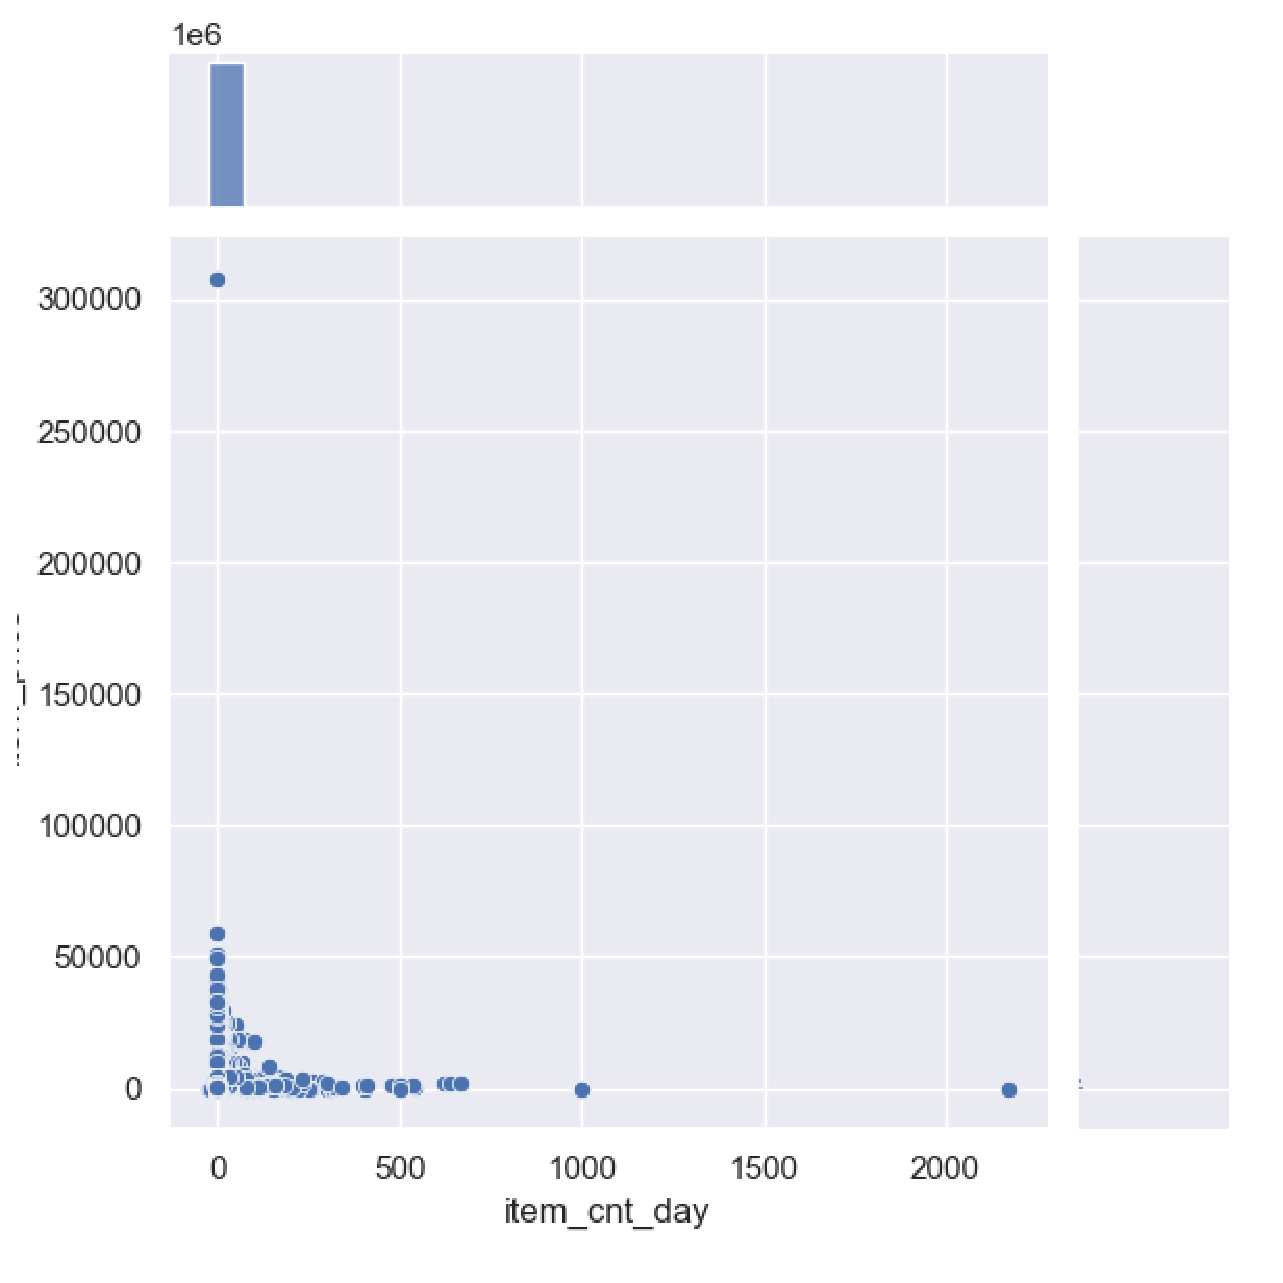
\includegraphics[width=0.9\textwidth]{logos/filter1.eps}
  %{\small{cost}}
  \end{minipage}
\end{center}
4.3 \textbf{Sales analysis}\\
%Firstly, for the overall analysis, we forecast from these aspects:\\
(1) Shows the store's total monthly sales and total sales per item.\\
Overall sales were down, and monthly sales were mostly down year on year.
One item sold exceptionally well.
\begin{center}
 
  \begin{minipage}{0.5\linewidth}
  \centering

  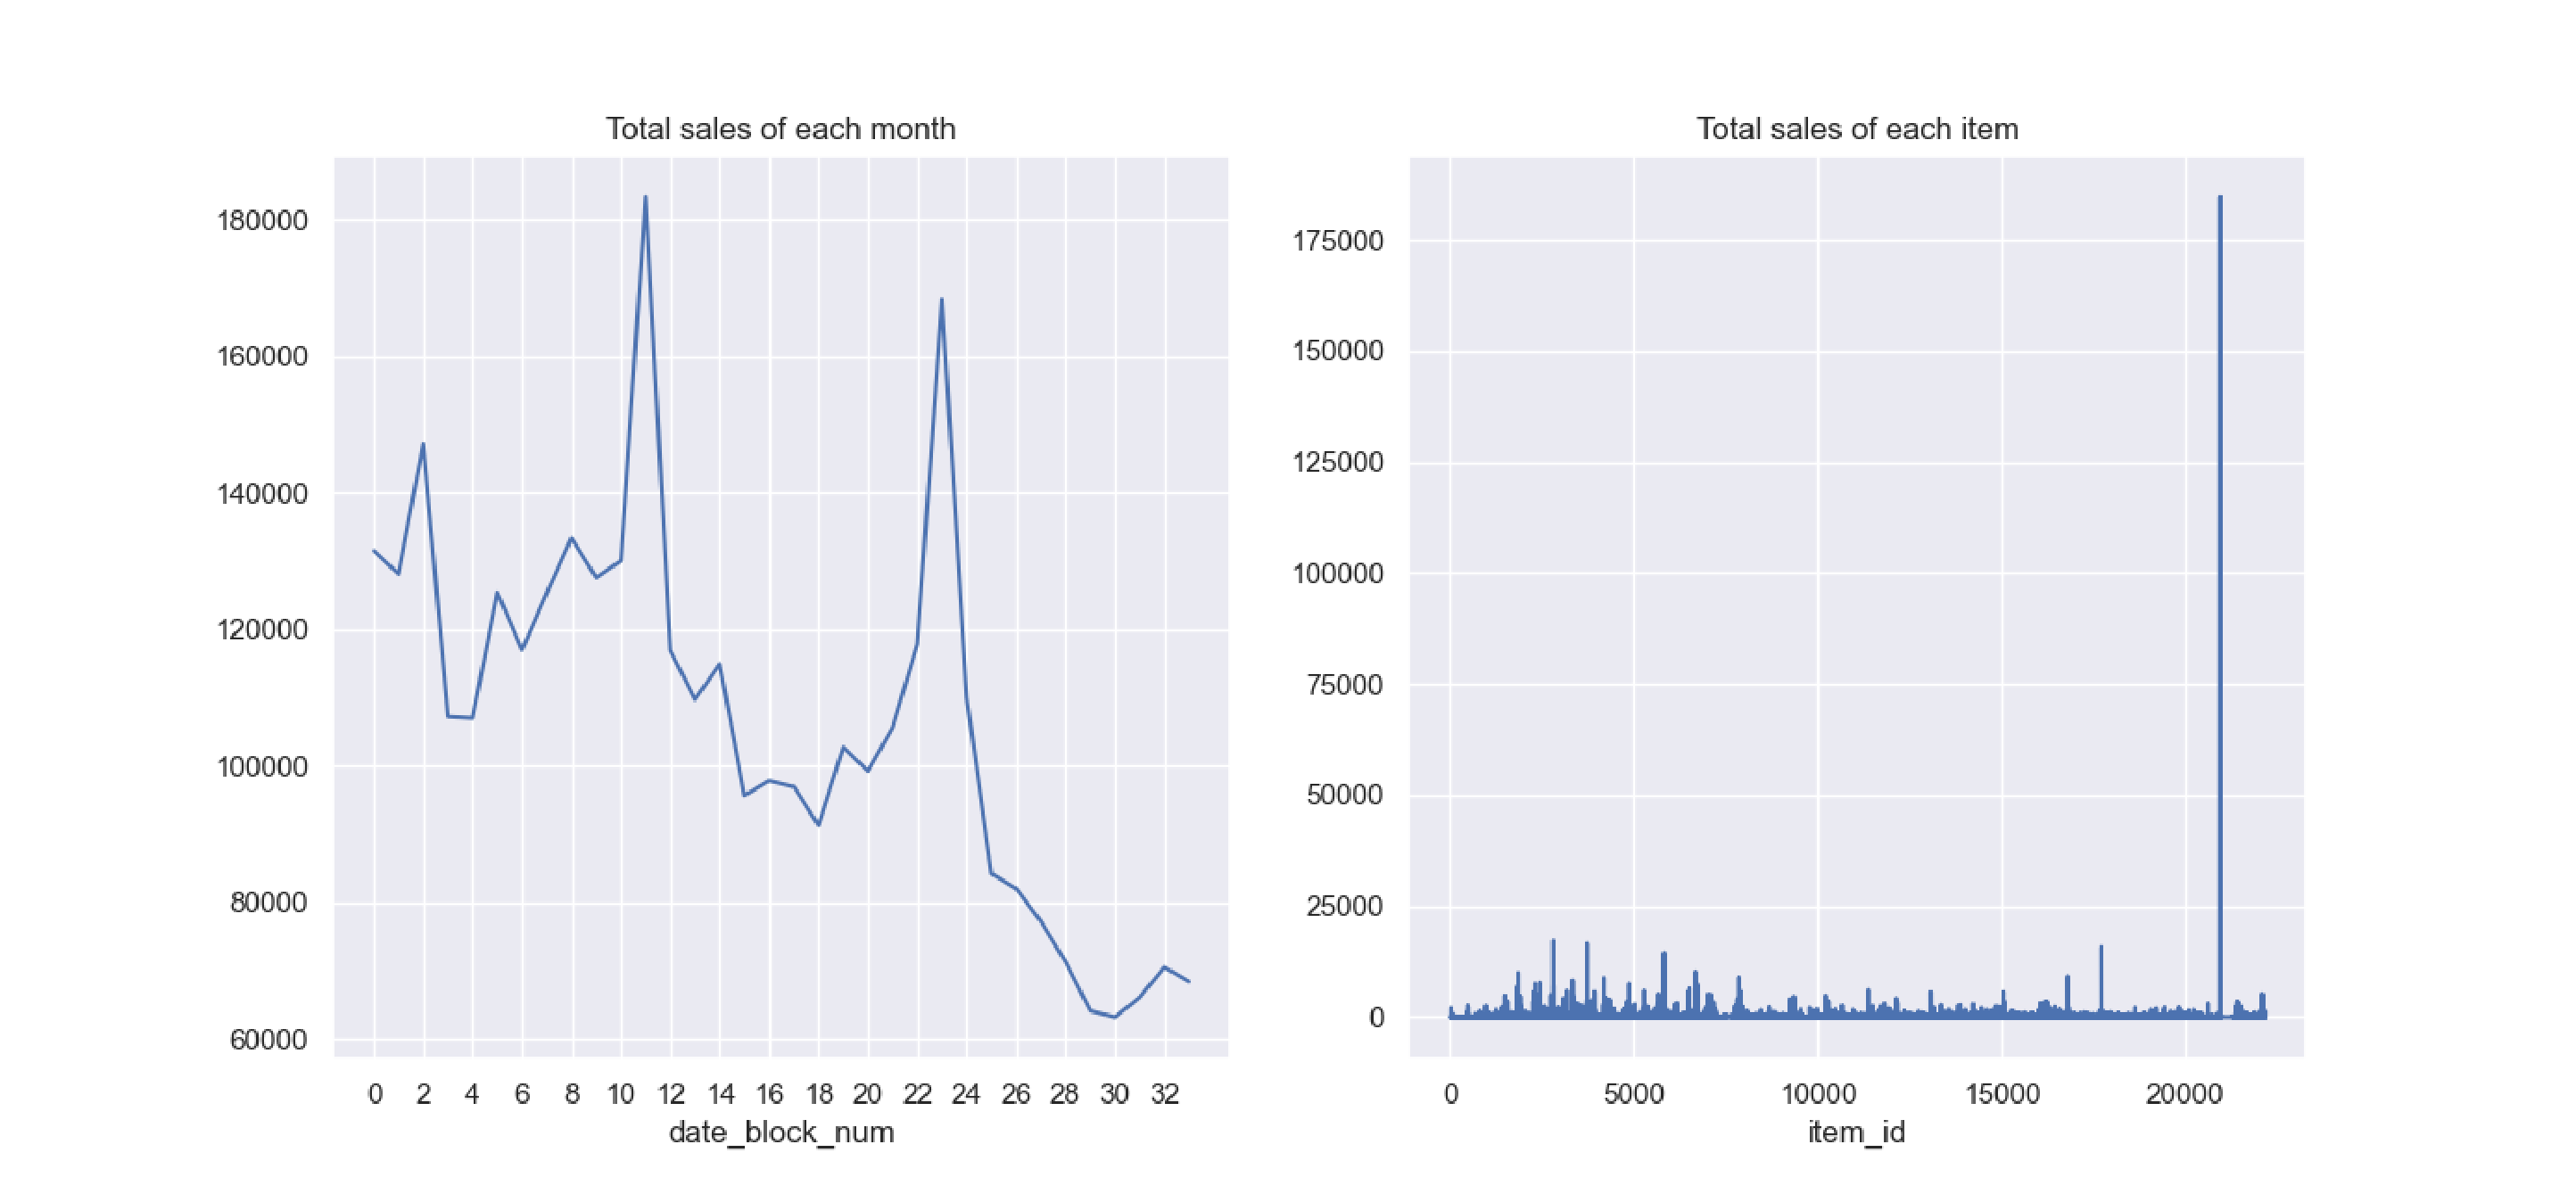
\includegraphics[width=1.1\textwidth]{logos/sale.eps}

  %{\small{cost}}

  \end{minipage}
\end{center}
(2) Monthly sales of the highest selling item.
\begin{center}

  \begin{minipage}{0.5\linewidth}
  \centering

  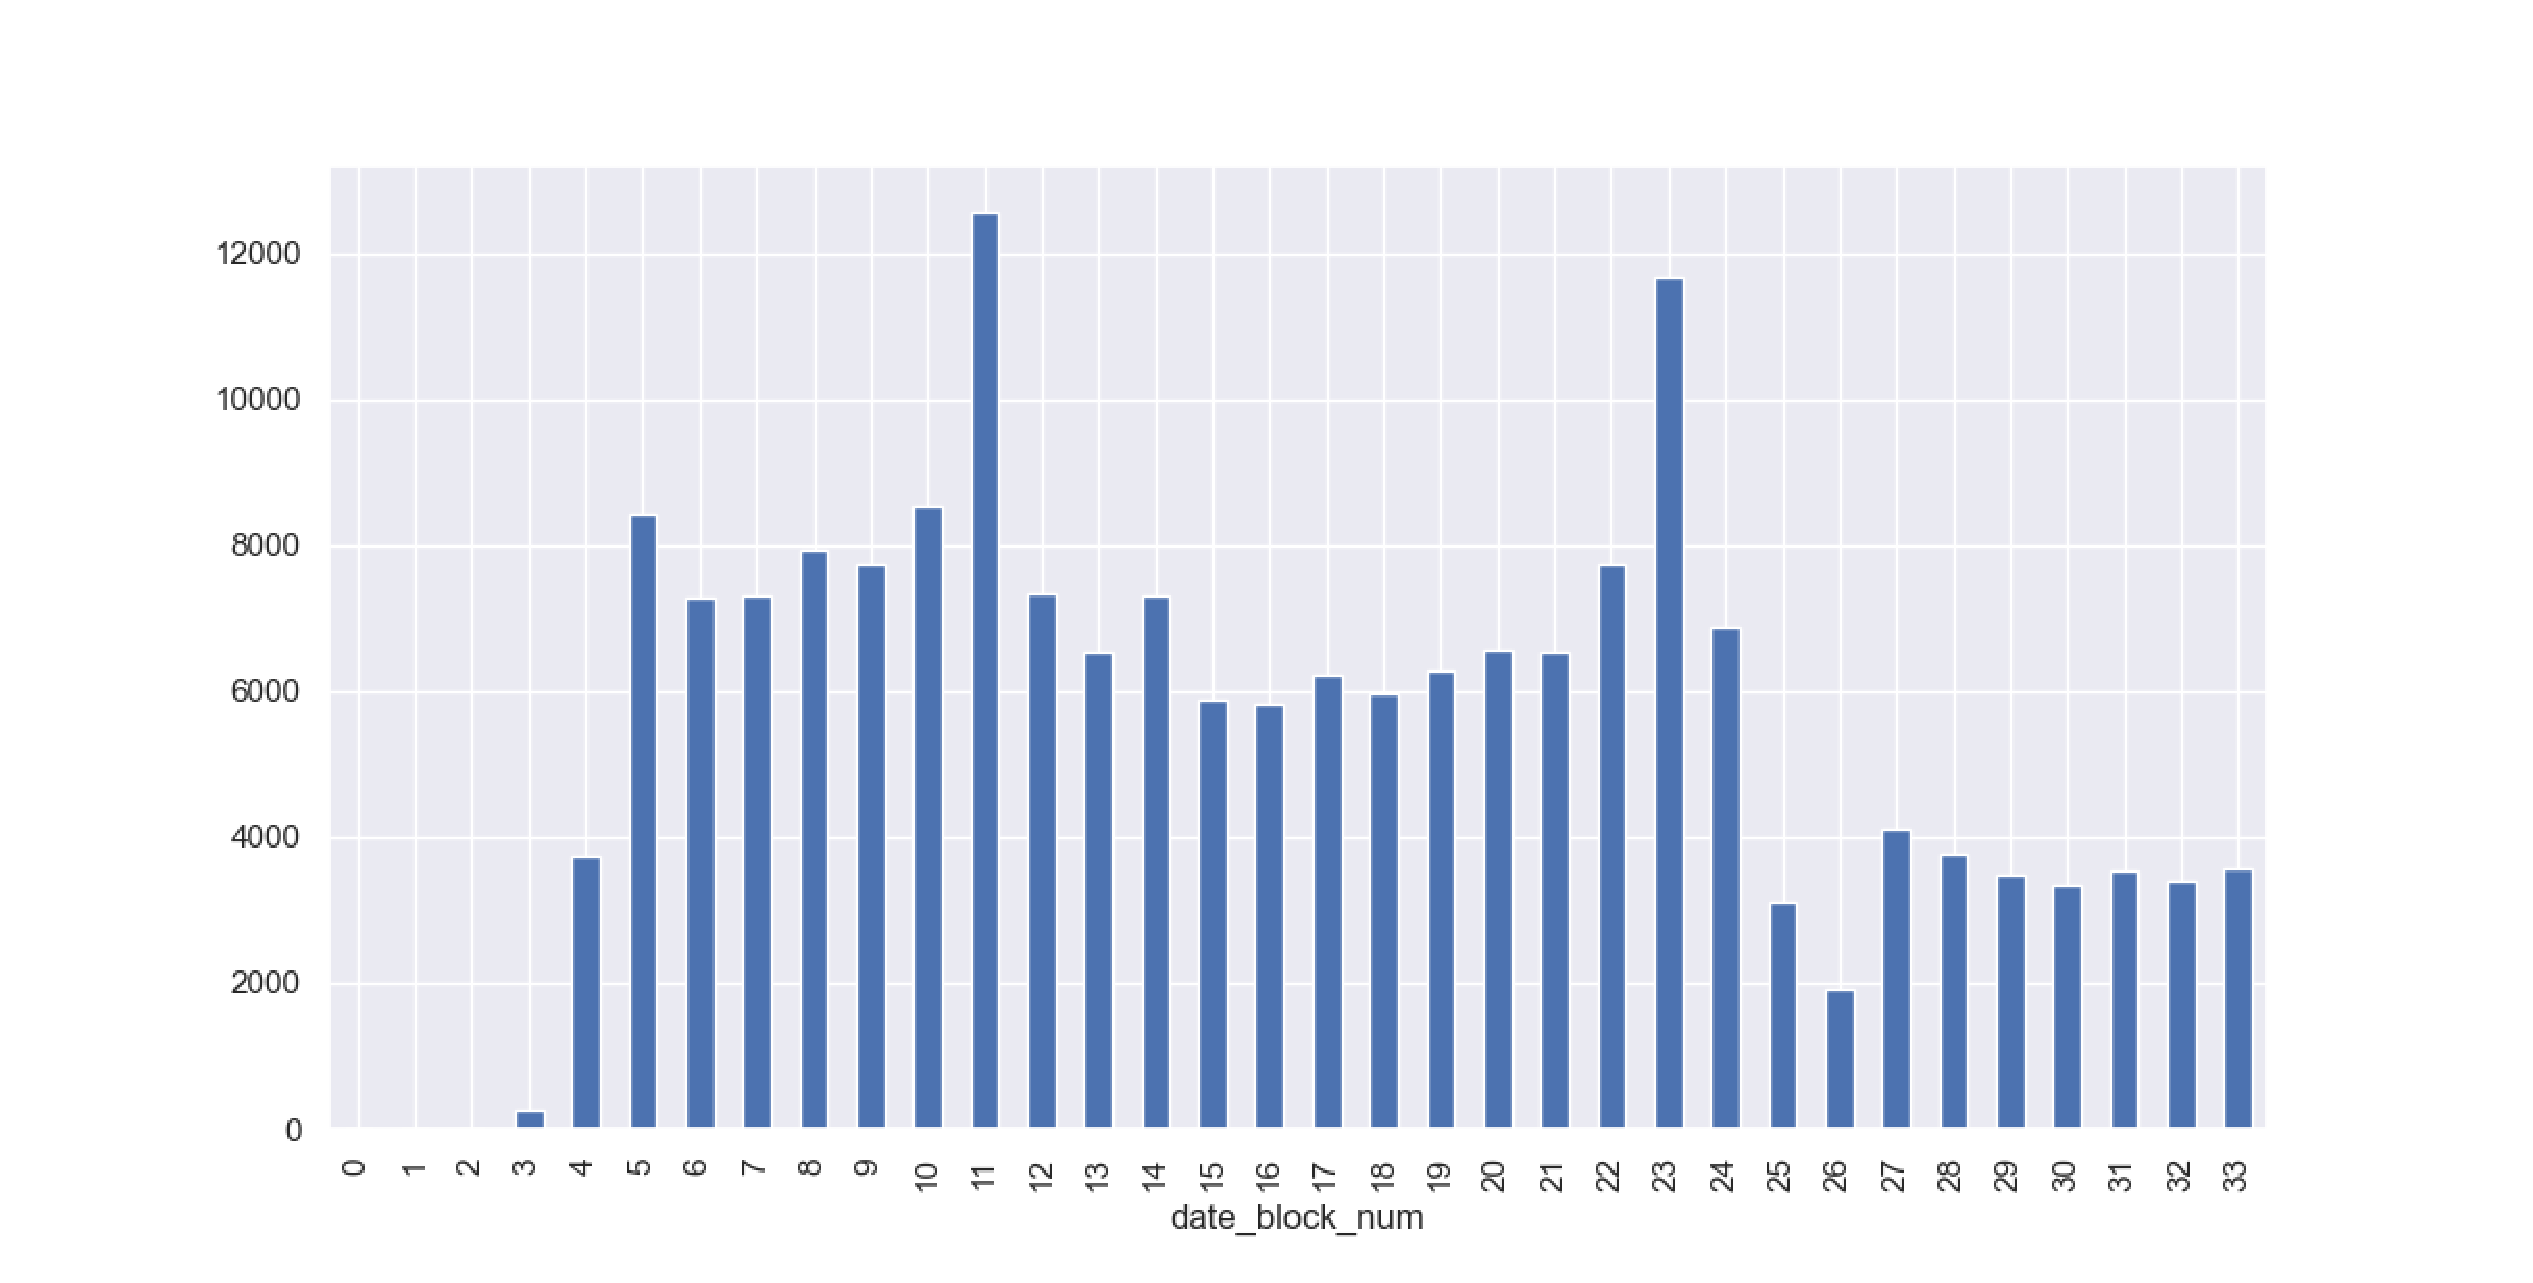
\includegraphics[width=1.1\textwidth]{logos/highite.eps}
  
  %{\small{cost}}

  \end{minipage}
\end{center}
(3) Shows the number of items sold each month.\\
The number of goods on sale shows an overall trend of continuous decline.\\
There are two possible reasons for the overall decline in monthly sales:\\
One is: the heat or life cycle of the goods in the store, and other internal factors related to the goods,\\
so that the sales volume of goods decreased.
Second, the goods are no longer sold due to external reasons such as withdrawal from shelves or shortage of goods,\\
thus affecting the sales volume of goods.
\begin{center}

  \begin{minipage}{0.5\linewidth}
  \centering

  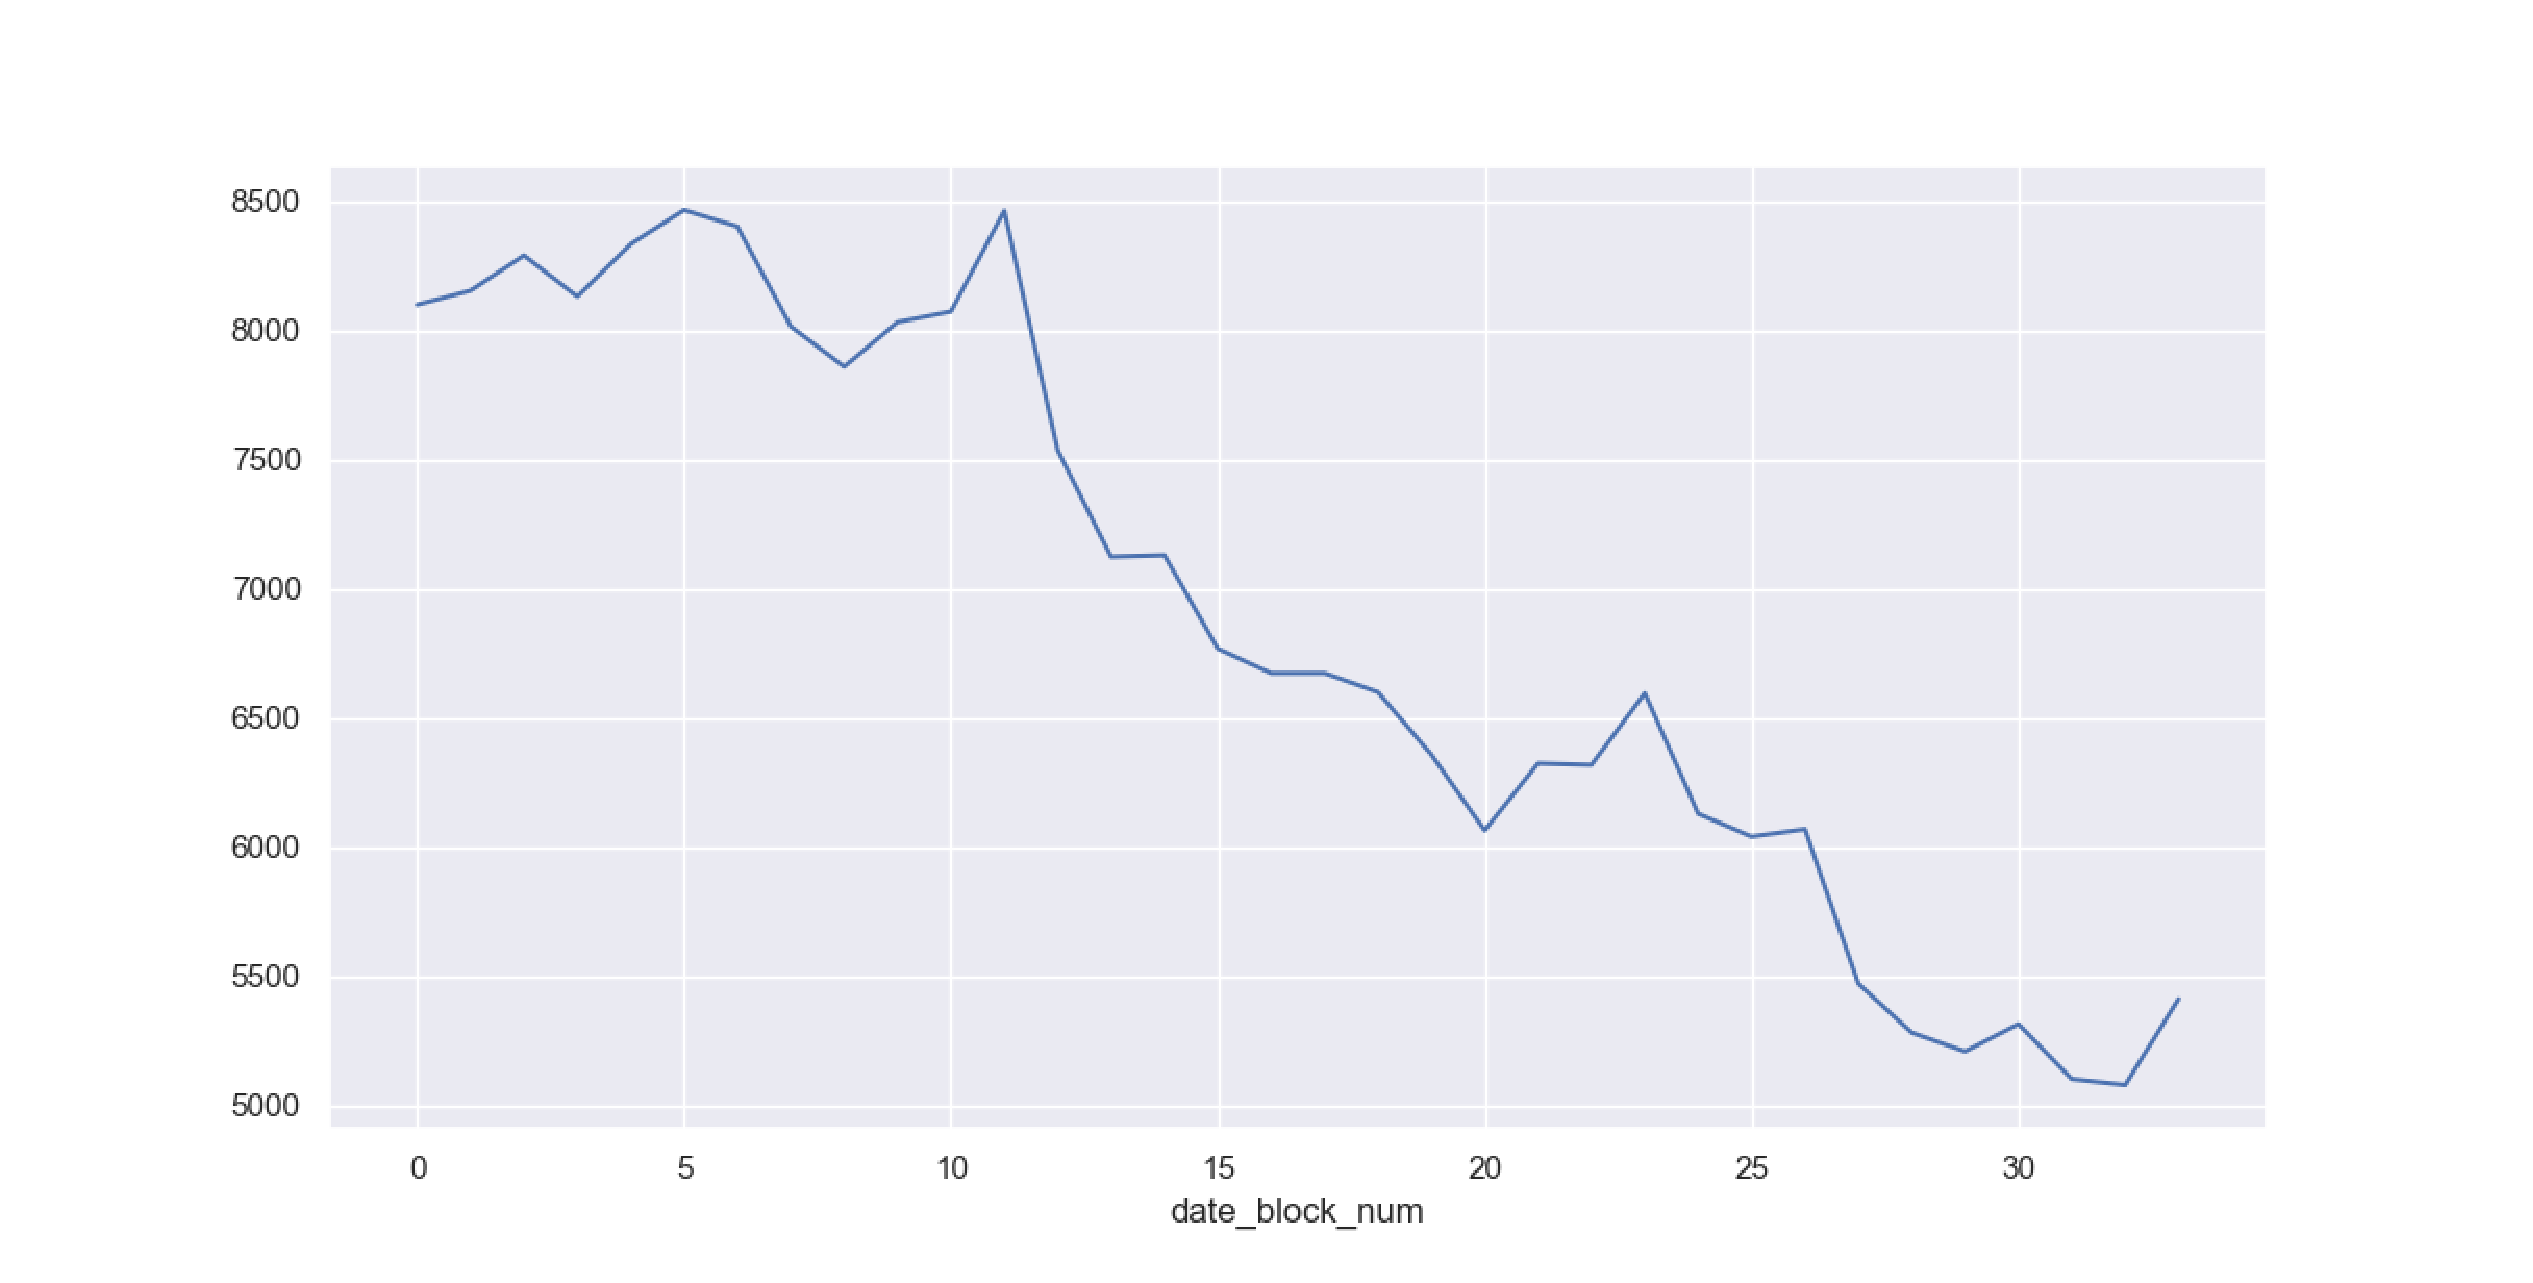
\includegraphics[width=1.1\textwidth]{logos/sloditem.eps}
  
  %{\small{cost}}

  \end{minipage}
\end{center}
4.4 \textbf{Revenue Analysis}\\
(1)Shows the company's total monthly revenue and total revenue per product.\\
Revenue in the 23rd month was up sharply from the 11th month, while sales were down year-on-year.\\
The e total revenue for one item was unusually high.\\
\begin{center}

  \begin{minipage}{0.5\linewidth}
  \centering

  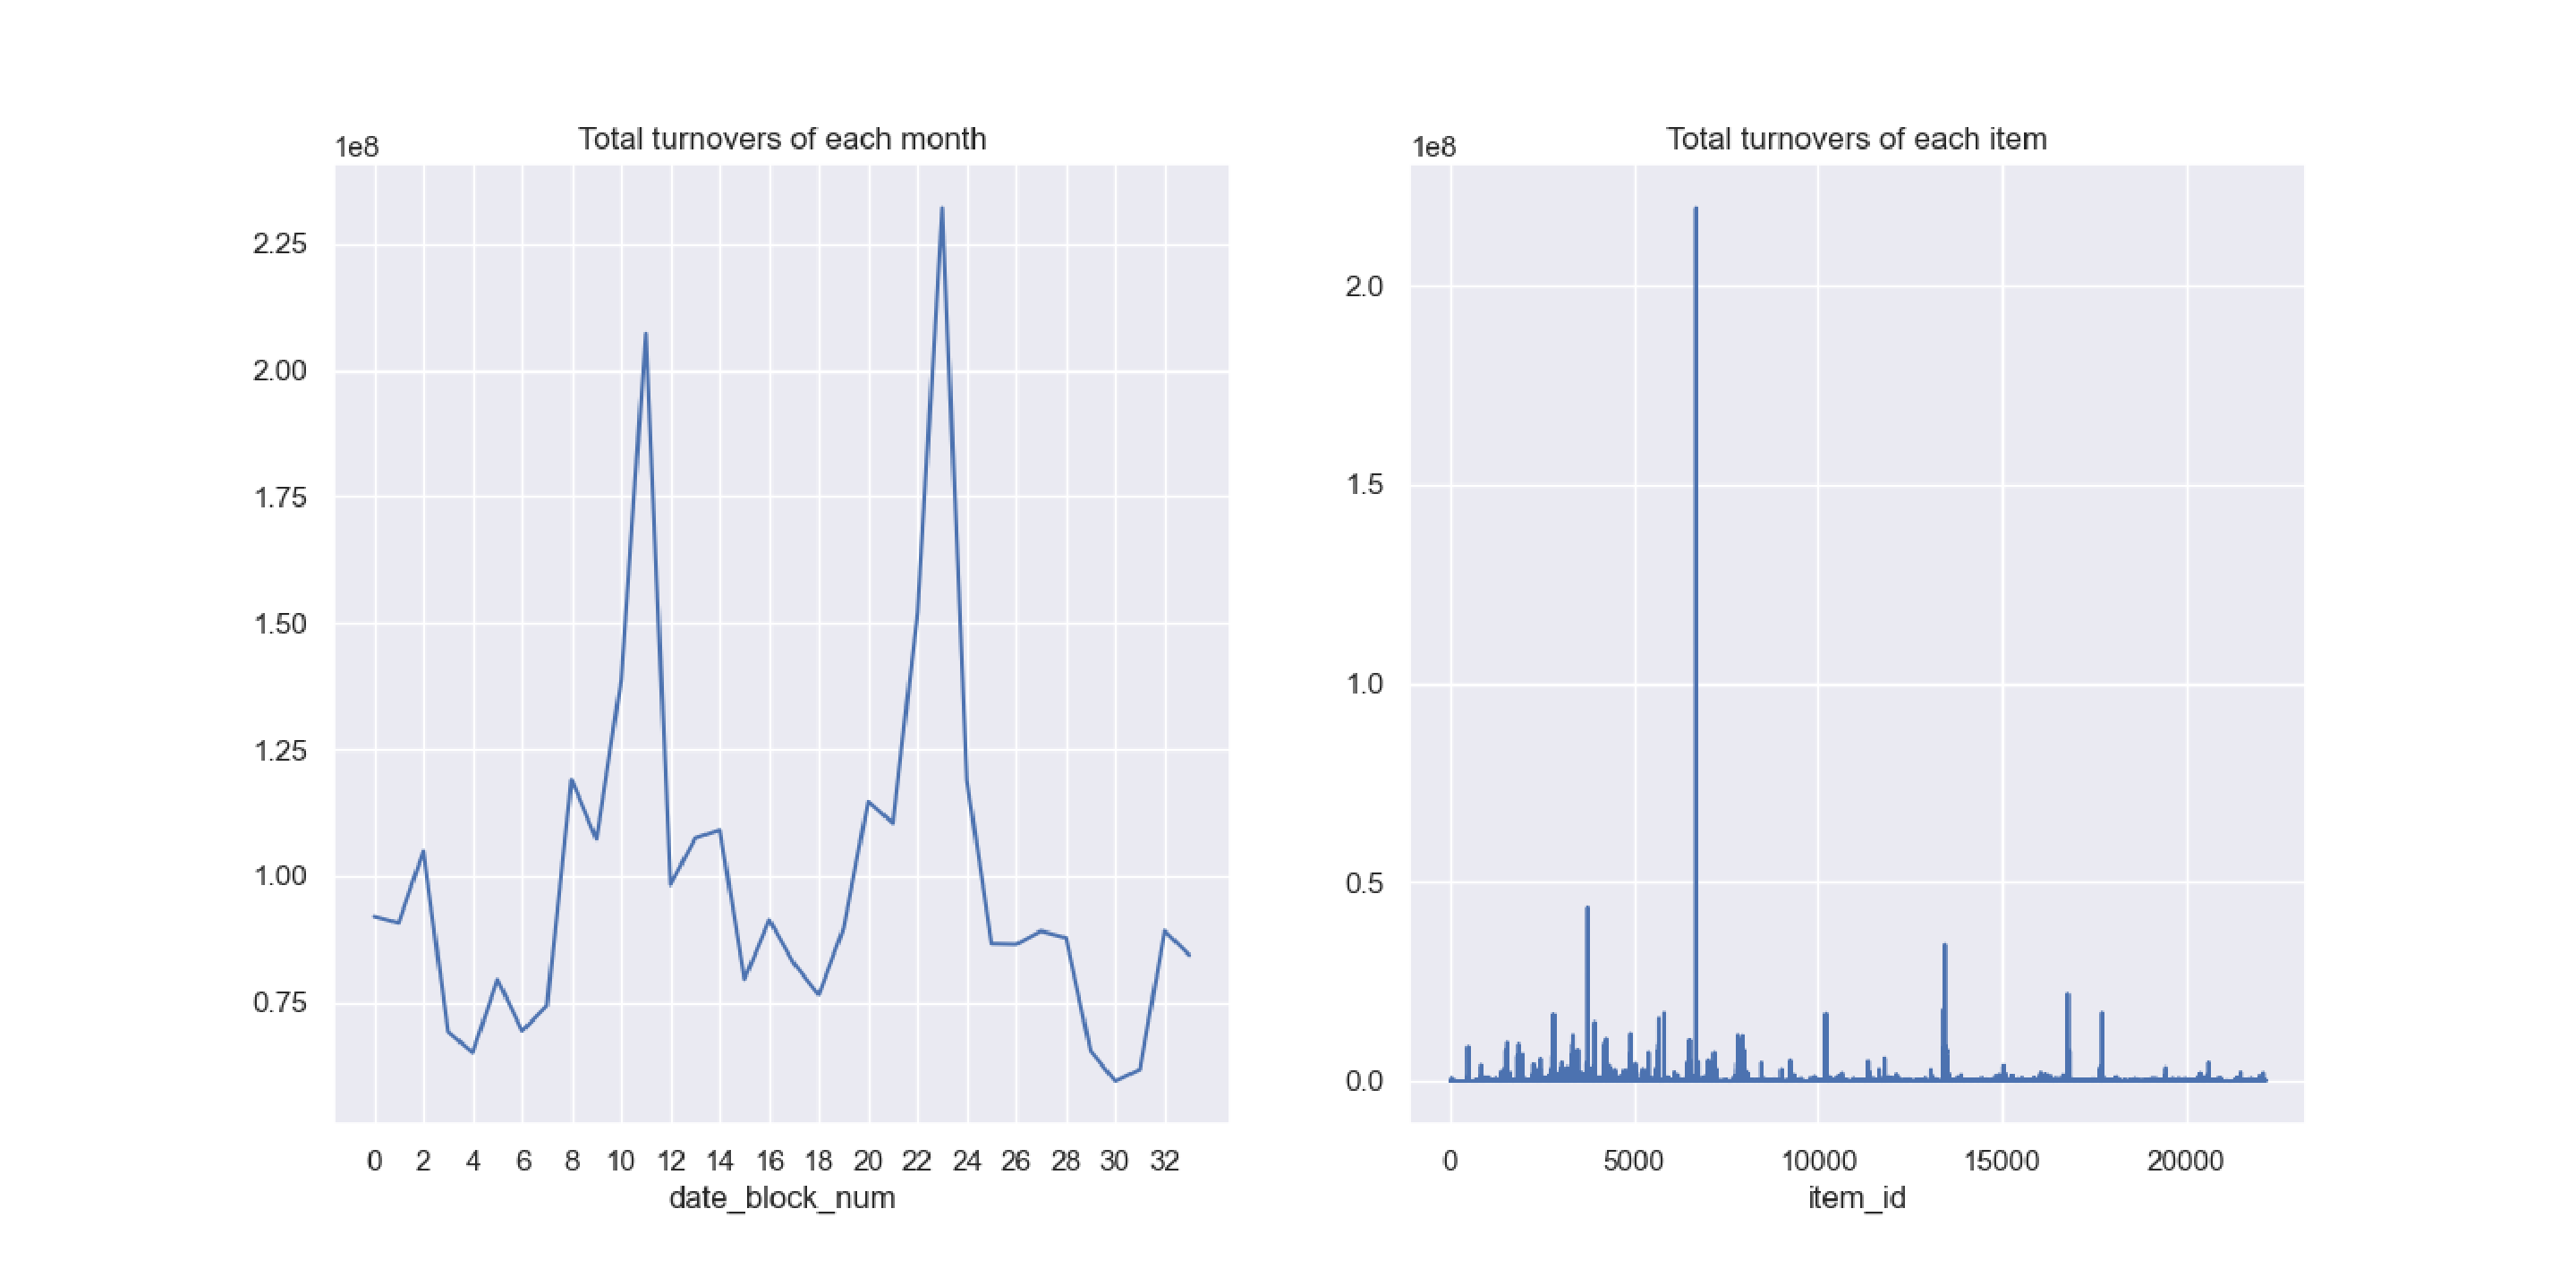
\includegraphics[width=1.1\textwidth]{logos/turnover.eps}
  
 % {\small{cost}}

  \end{minipage}

\end{center}
(2)Total revenue ranked no. 1 in merchandise sales per month.
% Revenue in the 23rd month was significantly higher than that in the 11th month, with an unusually high total revenue for one item.
\begin{center}

  \begin{minipage}{0.5\linewidth}
  \centering

  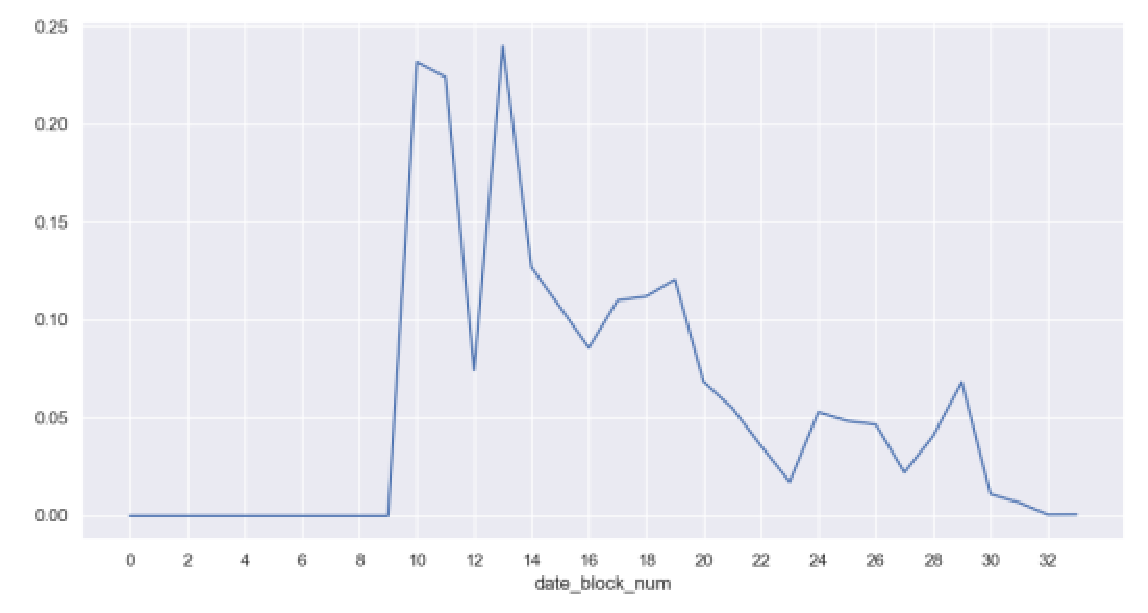
\includegraphics[width=1.1\textwidth]{logos/tuone.eps}
  
 % {\small{cost}}

  \end{minipage}
\end{center}

\indent 4.5 \textbf{Impact Analysis}\\
(1)The impact of the city in which the store is located on total revenue.\\
Stores in district 14 cities contributed the most to the total revenue.
\begin{center}

  \begin{minipage}{0.5\linewidth}
  \centering

  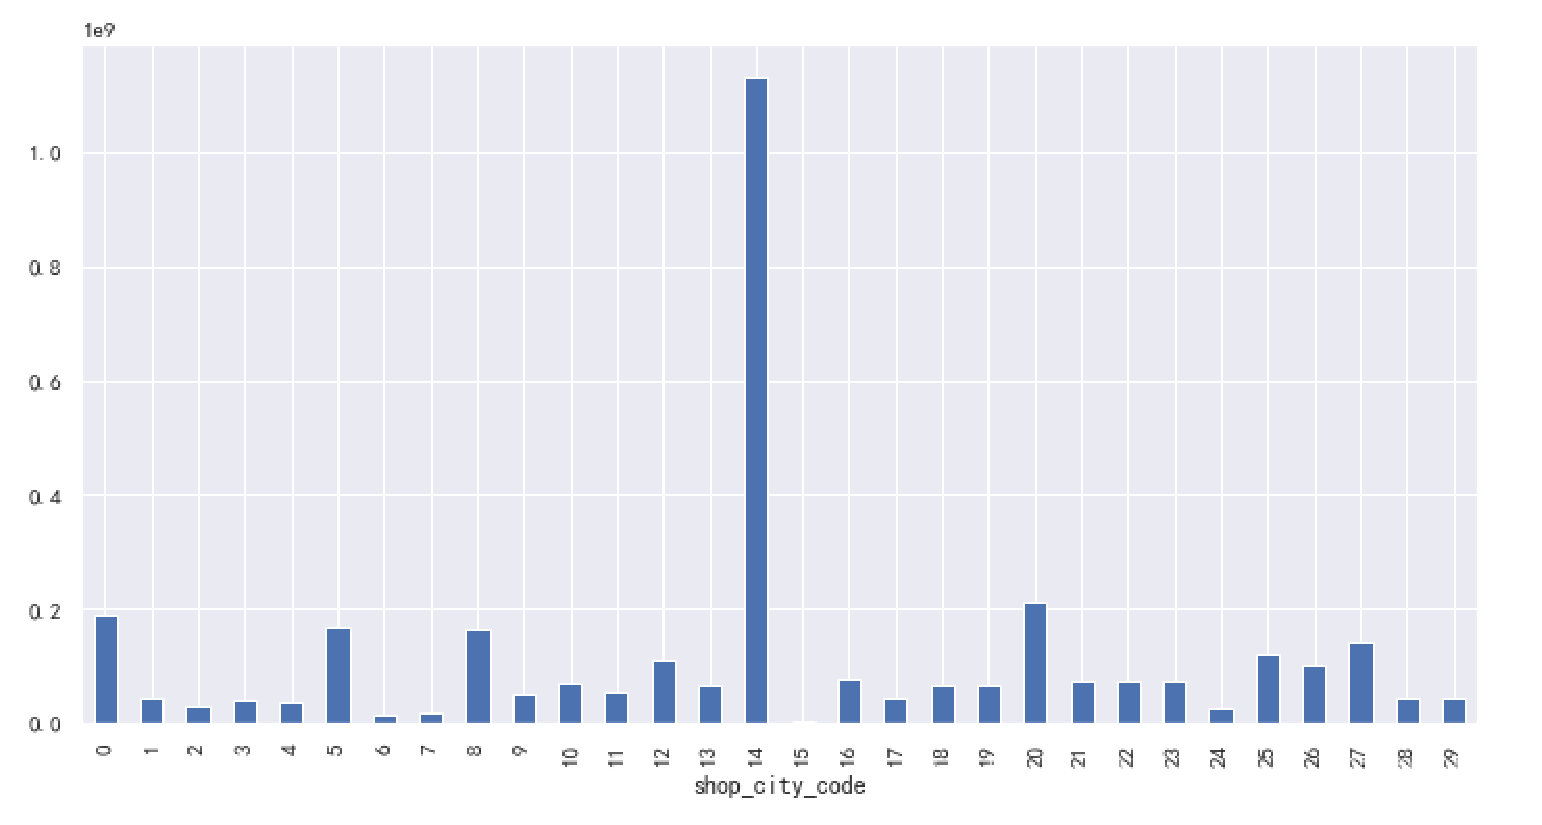
\includegraphics[width=1.1\textwidth]{logos/scity.eps}
  
 % {\small{cost}}

  \end{minipage}
\end{center}
(2)The impact of store type on total revenue\\
Category 1 stores contributed the most to total revenue.\\
\begin{center}

  \begin{minipage}{0.7\linewidth}
  \centering

  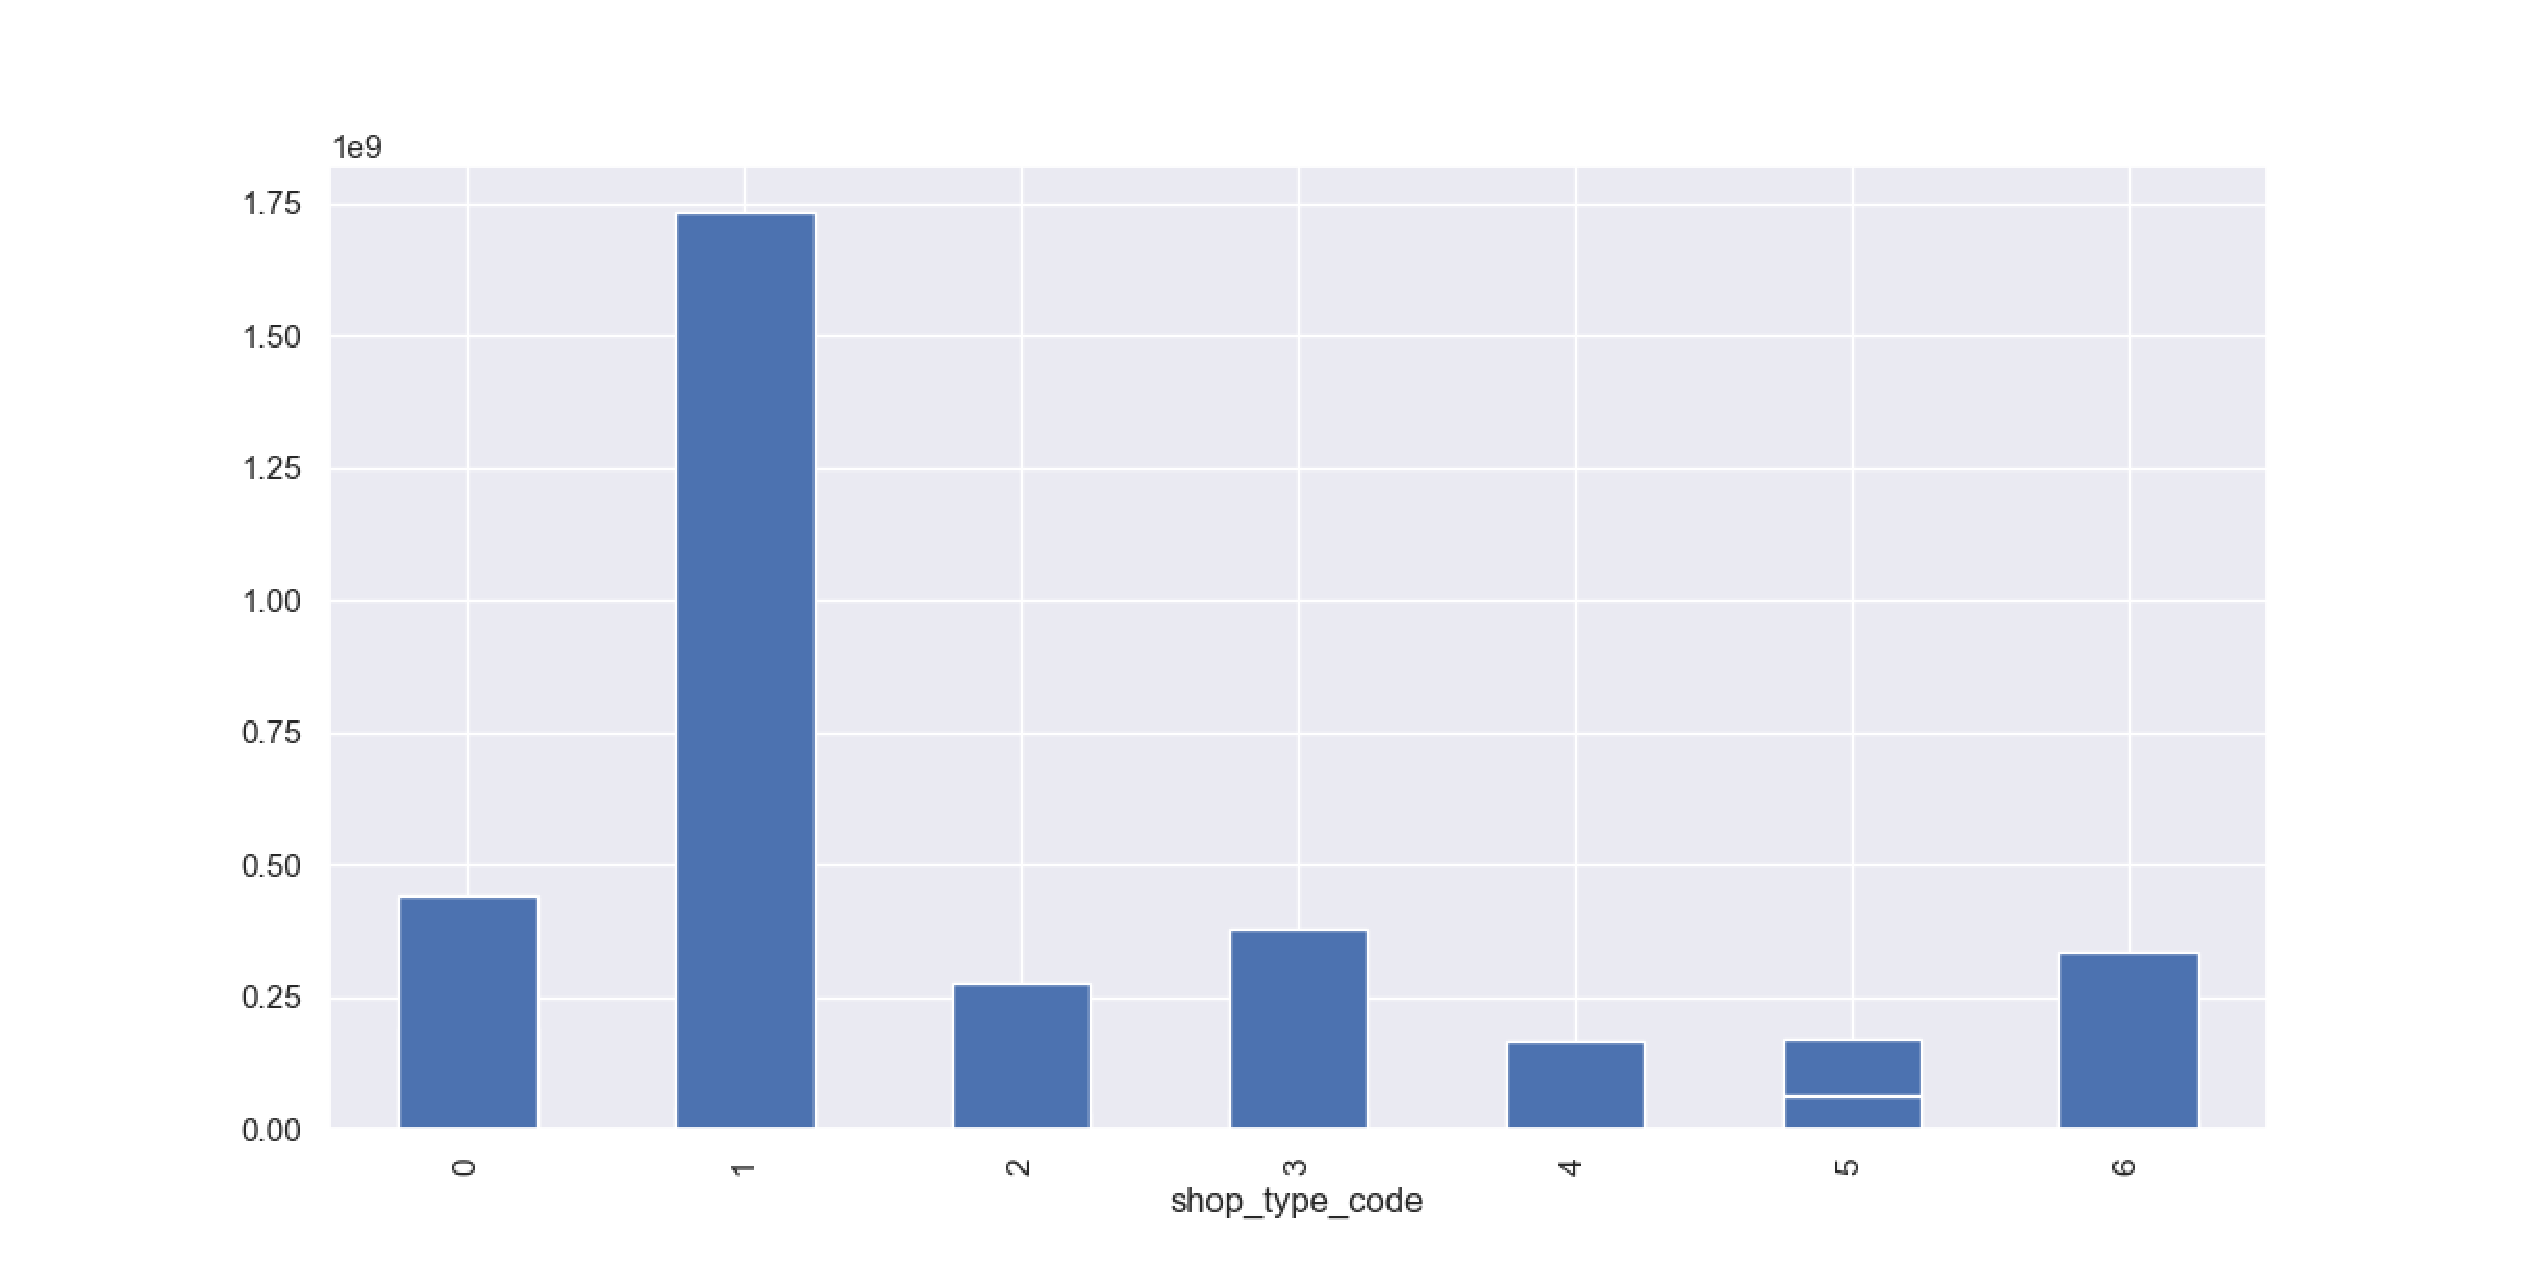
\includegraphics[width=1.0\textwidth]{logos/slei.eps}
  
 % {\small{cost}}

  \end{minipage}
\end{center}



\section{Conclusions}\label{sec-preliminaries}

Through this project, I have learned a lot, including the effective aspects of problem cutting, code implementation of analysis algorithm, design of analysis process, etc., which enables me to better grasp the thinking of data analysis on the whole.
%In feature processing, there is also a feature of the commodity price that is not added to the forecasting model.The main reason is that there are still some deficiencies in the treatment of price characteristics.
In the process of predictive analysis, the theoretical and data support for feature analysis and model construction is not concise and powerful enough, which needs to be strengthened.
